\appendix

\section{Comparison with \SB}\label{appendix:SB}

We compare the Padova+Geneva models with the \SB{} instantaneous bursts recommended by \citet{Levesque10} by running both sets of ionizing spectra through \Cloudy with identical parameters. The \SB{} models adopt similar ingredients, including the same high mass-loss rate evolutionary tracks from the Geneva group, described in \citet{Meynet00}, the BaSeL spectral library (\SB uses an earlier compilation, presented in \citet{Lejeune}) and the same spectral libraries for hot stars (WM-BASIC for O-type stars and and CMFGEN for WR stars, earlier versions).

We compare the resultant line ratios in \ref{fig:BPTsb99}, which show excellent agreement, as expected, since both models use the same isochrones and an almost identical combination of stellar libraries. The emission line ratios differ quantitatively by $\sim5-10\%$, but show the same qualitative behavior and overlap in much of parameter space. Emission line tables for the \SB models are available upon request.

%-------------------------------------------------------
% ISOCHRONES: SB99 BPT Age Evolution
%-------------------------------------------------------
\begin{figure}
  \begin{centering}
    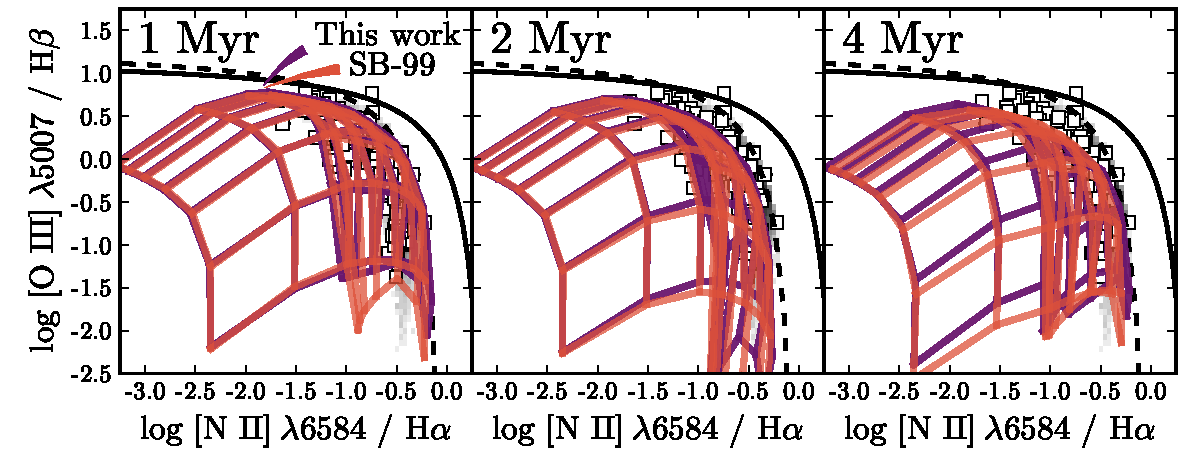
\includegraphics[width=0.75\textwidth]{manuscript/chapter2/f32.pdf}
    \caption{BPT diagram comparing line ratios from \Cloudy models run with ionizing spectra generated by two different SPS codes: FSPS and \SB. The models agree within $\sim5-10\%$ and show similar qualitative behavior.}
    \label{fig:BPTsb99}
  \end{centering}
\end{figure}
%-------------------------------------------------------

The set of \SB models from \citet{Levesque14} apply new Geneva tracks that include the effect of stellar rotation. Shown in \S\ref{sec:secondary:isochrones}, this has important implications on the time evolution of the BPT line ratios, and ultimately the lifetimes associated with ionization regions. A detailed study on the effects of stellar rotation on ionizing radiation and a full comparison between the \SB models with rotation and the MIST models (which include rotation) will be discussed in a future paper, Choi et al. (in prep).

\section{Emission Line List}\label{appendix:lines}
The list of emission lines in the \FSPS nebular model is included here.

%\startlongtable
\begin{deluxetable}{lll}
\tablecolumns{3}
\tablewidth{0pt}
\tabletypesize{\footnotesize}
\tablecaption{Emission lines included in the \FSPS nebular model\label{tab:emLines}}
\tablehead{
\colhead{Vacuum Wavelength (\ang)} &
\colhead{Line ID} &
\colhead{\Cloudy ID}\\
\colhead{} & \colhead{} & \colhead{}
}
\startdata
1215.6701 & H I (Ly-$\alpha$) & \texttt{H  1 1215.68A}\\
1025.728 & H I (Ly-$\beta$) & \texttt{H  1 1025.73A}\\
972.517 & H I (Ly-$\gamma$) & \texttt{H  1 972.543A}\\
949.742 & H I (Ly-$\delta$) & \texttt{H  1 949.749A}\\
937.814 & H I (Ly-5) & \texttt{H  1 937.809A}\\
930.751 & H I (Ly-6) & \texttt{H  1 930.754A}\\
926.249 & H I (Ly-7) & \texttt{H  1 926.231A}\\
923.148 & H I (Ly-8) & \texttt{H  1 923.156A}\\
6564.6 & H-$\alpha$ 6563 & \texttt{H  1 6562.85A}\\
4862.71 & H-$\beta$ 4861 & \texttt{H  1 4861.36A}\\
4341.692 & H-$\gamma$ 4340 & \texttt{H  1 4340.49A}\\
4102.892 & H-$\delta$ 4102 & \texttt{H  1 4101.76A}\\
3971.198 & H-5 3970 & \texttt{H  1 3970.09A}\\
3890.166 & H-6 3889 & \texttt{H  1 3889.07A}\\
3836.485 & H-7 3835 & \texttt{H  1 3835.40A}\\
3798.987 & H-8 3798 & \texttt{H  1 3797.92A}\\
18756.4 & H I (Pa-$\alpha$) & \texttt{H  1 1.87511m}\\
12821.578 & H I (Pa-$\beta$) & \texttt{H  1 1.28181m}\\
10941.17 & H I (Pa-$\gamma$) & \texttt{H  1 1.09381m}\\
10052.6 & H I (Pa-$\delta$) & \texttt{H  1 1.00494m}\\
9548.8 & H I (Pa-5) & \texttt{H  1 9545.99A}\\
9232.2 & H I (Pa-6) & \texttt{H  1 9229.03A}\\
9017.8 & H I (Pa-7) & \texttt{H  1 9014.92A}\\
40522.79 & H I (Br-$\alpha$) & \texttt{H  1 4.05116m}\\
26258.71 & H I (Br-$\beta$) & \texttt{H  1 2.62515m}\\
21661.178 & H I (Br-$\gamma$) & \texttt{H  1 2.16553m}\\
19450.89 & H I (Br-$\delta$) & \texttt{H  1 1.94456m}\\
18179.2 & H I (Br-5) & \texttt{H  1 1.81741m}\\
17366.885 & H I (Br-6) & \texttt{H  1 1.73621m}\\
74599.0 & H I (Pf-$\alpha$) & \texttt{H  1 7.45781m}\\
46537.8 & H I (Pf-$\beta$) & \texttt{H  1 4.65250m}\\
37405.76 & H I (Pf-$\gamma$) & \texttt{H  1 3.73953m}\\
32969.8 & H I (Pf-$\delta$) & \texttt{H  1 3.29609m}\\
30392.02 & H I (Pf-5) & \texttt{H  1 3.03837m}\\
123719.12 & H I (Hu-$\alpha$) & \texttt{H  1 12.3685m}\\
75024.4 & H I (Hu-$\beta$) & \texttt{H  1 7.50043m}\\
59082.2 & H I (Hu-$\gamma$) & \texttt{H  1 5.90659m}\\
51286.5 & H I (Hu-$\delta$) & \texttt{H  1 5.12725m}\\
4472.735 & He{\sc\,i} 4472 & \texttt{He 1 4471.47A}\\
5877.249 & He{\sc\,i} 5877 & \texttt{He 1 5875.61A}\\
6679.995 & He{\sc\,i} 6680 & \texttt{He 1 6678.15A}\\
10832.057 & He{\sc\,i} 10829 & \texttt{He 1 1.08299m}\\
10833.306 & He{\sc\,i} 10833 & \texttt{He 1 1.08303m}\\
3889.75 & He{\sc\,i} 3889 & \texttt{He 1 3888.63A}\\
7067.138 & He{\sc\,i} 7065 & \texttt{He 1 7065.18A}\\
1640.42 & He{\sc\,ii} 1640 & \texttt{He 2 1640.00A}\\
9852.96 & [C{\sc\,i}] 9850 & \texttt{TOTL 9850.00A}\\
8729.53 & [C{\sc\,i}] 8727 & \texttt{C  1 8727.00A}\\
4622.864 & [C{\sc\,i}] 4621 & \texttt{C  1 4621.00A}\\
6097000.0 & [C{\sc\,i}] 610$\mu\mathrm{m}$ & \texttt{C  1 609.200m}\\
3703700.0 & [C{\sc\,i}] 369$\mu\mathrm{m}$ & \texttt{C  1 369.700m}\\
1576429.62 & [C{\sc\,ii}] 157.7$\mu\mathrm{m}$ & \texttt{C  2 157.600m}\\
2325.4 & C{\sc\,ii}] 2326 & \texttt{C  2 2325.00A}\\
2324.21 & C{\sc\,ii}] 2326 & \texttt{C  2 2324.00A}\\
2328.83 & C{\sc\,ii}] 2326 & \texttt{C  2 2329.00A}\\
2327.64 & C{\sc\,ii}] 2326 & \texttt{C  2 2328.00A}\\
2326.11 & C{\sc\,ii}] 2326 & \texttt{C  2 2327.00A}\\
1908.73 & C{\sc\,iii}]  & \texttt{C  3 1910.00A}\\
1906.68 & [C{\sc\,iii}]  & \texttt{C  3 1907.00A}\\
5201.705 & [N{\sc\,i}] 5200 & \texttt{N  1 5200.00A}\\
6585.27 & [N{\sc\,ii}] 6585 & \texttt{N  2 6584.00A}\\
6549.86 & [N{\sc\,ii}] 6549 & \texttt{N  2 6548.00A}\\
5756.19 & [N{\sc\,ii}] 5756 & \texttt{N  2 5755.00A}\\
1218000.0 & [N{\sc\,ii}] 122$\mu\mathrm{m}$ & \texttt{N  2 121.700m}\\
2053000.0 & [N{\sc\,ii}] 205$\mu\mathrm{m}$ & \texttt{N  2 205.400m}\\
2142.3 & N{\sc\,ii}] 2141 & \texttt{N  2 2141.00A}\\
573300.0 & [N{\sc\,iii}] 57$\mu\mathrm{m}$ & \texttt{N  3 57.2100m}\\
6302.046 & [O{\sc\,i}] 6302 & \texttt{O  1 6300.00A}\\
6365.535 & [O{\sc\,i}] 6365 & \texttt{O  1 6363.00A}\\
5578.89 & [O{\sc\,i}] 5578 & \texttt{O  1 5577.00A}\\
631852.0 & [O{\sc\,i}] 63$\mu\mathrm{m}$ & \texttt{O  1 63.1700m}\\
1455350.0 & [O{\sc\,i}] 145$\mu\mathrm{m}$ & \texttt{O  1 145.530m}\\
3727.1 & [O{\sc\,ii}] 3726 & \texttt{O II 3726.00A}\\
3729.86 & [O{\sc\,ii}] 3729 & \texttt{O II 3729.00A}\\
7332.21 & [O{\sc\,ii}] 7332 & \texttt{O II 7332.00A}\\
7321.94 & [O{\sc\,ii}] 7323 & \texttt{O II 7323.00A}\\
2471.088 & [O{\sc\,ii}] 2471 & \texttt{O II 2471.00A}\\
1661.241 & O{\sc\,iii}] 1661 & \texttt{O  3 1661.00A}\\
1666.15 & O{\sc\,iii}] 1666 & \texttt{O  3 1666.00A}\\
5008.24 & [O{\sc\,iii}] 5007 & \texttt{O  3 5007.00A}\\
4960.295 & [O{\sc\,iii}] 4960 & \texttt{O  3 4959.00A}\\
4364.435 & [O{\sc\,iii}] 4364 & \texttt{TOTL 4363.00A}\\
2321.664 & [O{\sc\,iii}] 2321 & \texttt{O  3 2321.00A}\\
883564.0 & [O{\sc\,iii}] 88$\mu\mathrm{m}$ & \texttt{O  3 88.3300m}\\
518145.0 & [O{\sc\,iii}] 52$\mu\mathrm{m}$ & \texttt{O  3 51.8000m}\\
128135.48 & [Ne{\sc\,ii}] 12.8$\mu\mathrm{m}$ & \texttt{Ne 2 12.8100m}\\
155551.0 & [Ne{\sc\,iii}] 15.5$\mu\mathrm{m}$ & \texttt{Ne 3 15.5500m}\\
360135.0 & [Ne{\sc\,iii}] 36$\mu\mathrm{m}$ & \texttt{Ne 3 36.0140m}\\
3869.86 & [Ne{\sc\,iii}] 3870 & \texttt{Ne 3 3869.00A}\\
3968.59 & [Ne{\sc\,iii}] 3968 & \texttt{Ne 3 3968.00A}\\
3343.5 & [Ne{\sc\,iii}] 3343 & \texttt{Ne 3 3343.00A}\\
1812.205 & [Ne{\sc\,iii}] 1815 & \texttt{Ne 3 1815.00A}\\
4725.47 & [Ne{{\sc\,iv}}] 4720 & \texttt{Ne 4 4720.00A}\\
2796.352 & Mg{\sc\,ii} 2800 & \texttt{Mg 2 2795.53A}\\
2803.53 & Mg{\sc\,ii} 2800 & \texttt{Mg 2 2802.71A}\\
348140.0 & [Si{\sc\,ii}] 35$\mu\mathrm{m}$ & \texttt{Si 2 34.8140m}\\
10323.32 & [S{\sc\,ii}] 10331 & \texttt{S  2 1.03300m}\\
6732.673 & [S{\sc\,ii}] 6732 & \texttt{S II 6731.00A}\\
6718.294 & [S{\sc\,ii}] 6717 & \texttt{S II 6716.00A}\\
4069.75 & [S{\sc\,ii}] 4070 & \texttt{S II 4070.00A}\\
4077.5 & [S{\sc\,ii}] 4078 & \texttt{S II 4078.00A}\\
187130.0 & [S{\sc\,iii}] 18.7$\mu\mathrm{m}$ & \texttt{S  3 18.6700m}\\
334800.0 & [S{\sc\,iii}] 33.5$\mu\mathrm{m}$ & \texttt{S  3 33.4700m}\\
9533.2 & [S{\sc\,iii}] 9533 & \texttt{S  3 9532.00A}\\
9071.1 & [S{\sc\,iii}] 9071 & \texttt{S  3 9069.00A}\\
6313.81 & [S{\sc\,iii}] 6314 & \texttt{S  3 6312.00A}\\
3722.75 & [S{\sc\,iii}] 3723 & \texttt{S  3 3722.00A}\\
105105.0 & [S{{\sc\,iv}}] 10.5$\mu\mathrm{m}$ & \texttt{S  4 10.5100m}\\
69852.74 & [Ar{\sc\,ii}] 7$\mu\mathrm{m}$ & \texttt{Ar 2 6.98000m}\\
7137.77 & [Ar{\sc\,iii}] 7138 & \texttt{Ar 3 7135.00A}\\
7753.19 & [Ar{\sc\,iii}] 7753 & \texttt{Ar 3 7751.00A}\\
5193.27 & [Ar{\sc\,iii}] 5193 & \texttt{Ar 3 5192.00A}\\
3109.98 & [Ar{\sc\,iii}] 3110 & \texttt{Ar 3 3109.00A}\\
218302.0 & [Ar{\sc\,iii}] 22$\mu\mathrm{m}$ & \texttt{Ar 3 21.8300m}\\
89913.8 & [Ar{\sc\,iii}] 9$\mu\mathrm{m}$ & \texttt{Ar 3 9.00000m}\\
7334.17 & [Ar{{\sc\,iv}}] 7330 & \texttt{Ar 4 7331.00A}\\
2669.951 & [Al{\sc\,ii}] 2670 & \texttt{Al 2 2670.00A}\\
2661.146 & [Al{\sc\,ii}] 2660 & \texttt{Al 2 2660.00A}\\
1854.716 & [Al{\sc\,iii}] 1855 & \texttt{Al 3 1855.00A}\\
1862.7895 & [Al{\sc\,iii}] 1863 & \texttt{Al 3 1863.00A}\\
143678.0 & [Cl{\sc\,ii}] 14.4$\mu\mathrm{m}$ & \texttt{Cl 2 14.4000m}\\
8581.06 & [Cl{\sc\,ii}] 8579 & \texttt{Cl 2 8579.00A}\\
9126.1 & [Cl{\sc\,ii}] 9124 & \texttt{Cl 2 9124.00A}\\
5539.411 & [Cl{\sc\,iii}] 5538 & \texttt{Cl 3 5538.00A}\\
5519.242 & [Cl{\sc\,iii}] 5518 & \texttt{Cl 3 5518.00A}\\
606420.0 & [P{\sc\,ii}] 60$\mu\mathrm{m}$ & \texttt{P  2 60.6400m}\\
328709.0 & [P{\sc\,ii}] 32$\mu\mathrm{m}$ & \texttt{P  2 32.8700m}\\
12570.21 & [Fe{\sc\,ii}] 1.26$\mu\mathrm{m}$ & \texttt{Fe 2 1.25668m}\\
\enddata
\end{deluxetable}
